\chapter{LGR variations} %This title needs fixing

\section{Smaller Cavity LGR} \label{smallLGR}
\begin{figure}[b!]
\centering
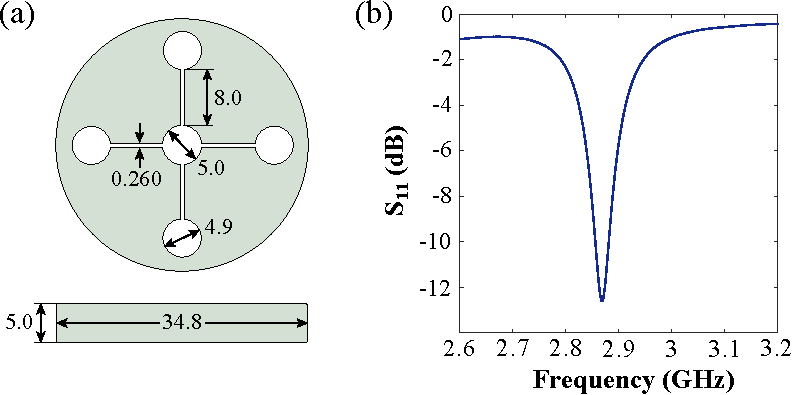
\includegraphics[width = \textwidth]{Figure_B_3.pdf}  
\caption{\textbf{Smaller LGR design} \textbf{(a)} Line drawing of smaller LGR with central loop radius $r_c = 2.5$ mm as described in section \ref{smallLGR}. Units are in mm. \textbf{(b)} Measured $S_{11}$ for composite device tuned to $f_0 \approx 2.87 GHz$.}
\label{smallLGRfigure}
\end{figure}   
To achieve stronger MW driving, we also designed and fabricated
smaller LGR with central loop radius $r_c = 2.5$ mm and $n = 4$ outer loops of radius $r_o = 2.45$ mm, as shown in Figure \ref{smallLGRfigure}. The naked air-gapped LGR cavity exhibits $f_0 = 4.5$ GHz, similar to the larger LGR design described in the main text. Employing the same exciter antenna, $B_1 = 5.8$ gauss is measured at the center of the smaller LGR device. The measured 3 dB bandwidth $\Delta_{3dB} = 112$ MHz corresponds to a loaded quality factor of $Q_L = 25.4$, and an associated ring-down time of 2.8 ns.


\begin{figure}[t!]
\centering
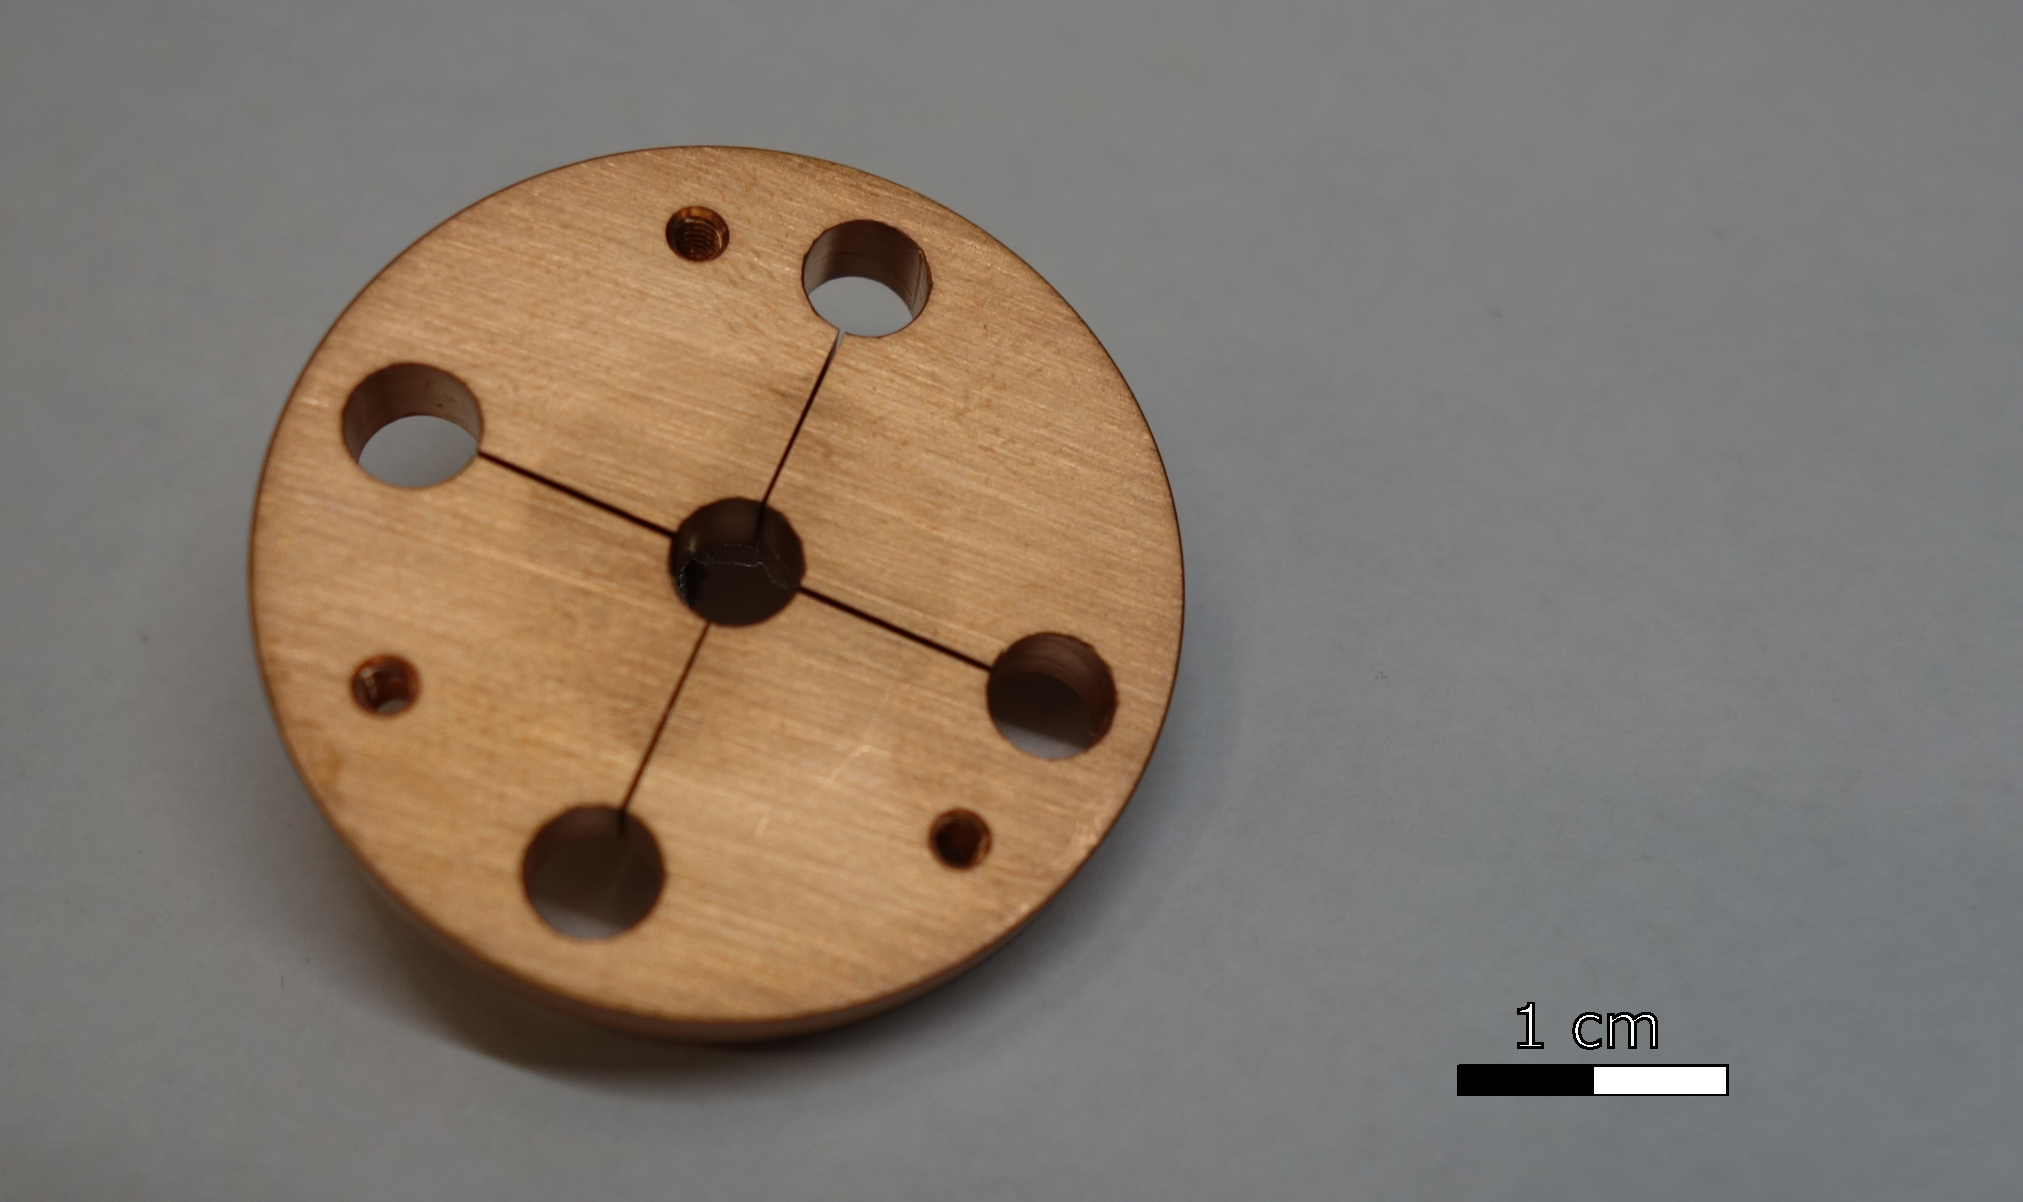
\includegraphics[width = \textwidth]{CopperLGR.pdf}  
\caption{\textbf{Copper Loop Gap Resonator} Loop Gap Resonator manufactured from C145 machinable copper}
\label{LGR_Copper}
\end{figure}   


\section{Copper LGR} \label{CopperLGR}

To achieve higher Q-factors without redesigning the LGR geometry one can fabricate the device from a more conductive material such as copper ($\sigma_c = 59 \times 10^6$ S/m). We manufactured an LGR in C145 machinable copper [Figure \ref{LGR_Copper}]. Figure \ref{LGR_Coppervstit} plots the reflection coefficient $S_{11}$ of both the copper and titanium LGR. Both are critically coupled and the Q factor (for the copper LGR) is measured to be 287, a $>\times 10$ improvement over the titanium device. Such an LGR can be desirable when bandwidth is not a limiting factor and stronger fields are required. The copper LGR has the same dimensions as the smaller cavity LGR in section \ref{smallLGR} that exhibits a Q of 25.4. Re-scaling the measured $B_1$ in the LGR center by $\sqrt{287}/\sqrt{25.4}$ yields the theoretical field strength in the center of the copper resonator. In this case the copper resonator is predicted to have a $B_1$ field strength of $\sim 19.5$ gauss in the center of the center loop.  

\begin{figure}[t!]
\centering
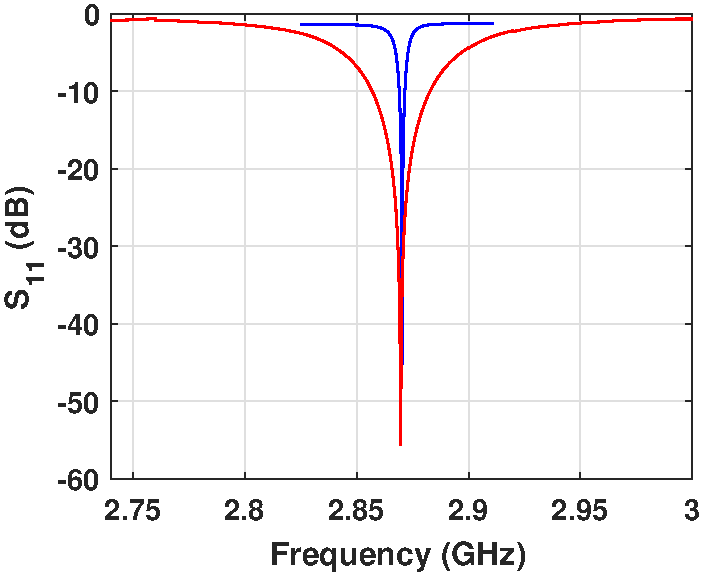
\includegraphics[scale = 0.85]{copperVStitanium.pdf}  
\caption{\textbf{Copper vs. Titanium LGR} Scattering parameters ($S_{11}$) of the copper manufactured LGR (\textcolor{blue}{---}) in comparison to titanium LGR (\textcolor{red}{---})}
\label{LGR_Coppervstit}
\end{figure} 

\section{Shielding}  

Fields that extended away from the LGR (ie. fields that aren't fully caught by the flux return loops) as well as fringing fields above and below the resonator can lead to handshaking or radiation losses if the resonator is not properly shielded during operation. However, because shielding limits the optical accessibility of the center loop and because bandwidth optimization is not the primary concern for the LGR's use as a MW drive source for NVs, shielding was not addressed during the experiment outlined in section \ref{measurement}. For the sake of completeness however, it should be mentioned that proper lateral shielding of the LGR can increase Q factors by minimizing the aforementioned loss mechanisms \cite{petryakov2001bridged, rinard2005loopgap}. Using a copper tube approximately $\times 1.5$ the full diameter of the LGR, an almost doubling of the LGR Q factor (from 287 to $\sim 470$) was achieved. Applying the same calculation as above, a $B_1$ field strength of $\sim 25$ gauss is expected when the copper resonator is properly shielded.   

\clearpage
\newpage
